\documentclass[journal=jctcce]{achemso}
\usepackage[version=3]{mhchem} 
\usepackage[T1]{fontenc}       
\newcommand*\mycommand[1]{\texttt{\emph{#1}}}
\usepackage{xcolor}
\usepackage{booktabs}
\usepackage{xr}
\usepackage{multirow}

\makeatletter
\newcommand*{\addFileDependency}[1]{% argument=file name and extension
  \typeout{(#1)}
  \@addtofilelist{#1}
  \IfFileExists{#1}{}{\typeout{No file #1.}}
}
\makeatother

\newcommand*{\myexternaldocument}[1]{%
    \externaldocument{#1}%
    \addFileDependency{#1.tex}%
    \addFileDependency{#1.aux}%
}
\myexternaldocument{manuscriptSUPPL}

\author{Fernando Favela-Rosales}
\affiliation{Departamento de F\'isica, Centro de Investigaci\'on y de Estudios Avanzados del IPN, Apartado Postal 14-740, 07000 M\'exico D.F., M\'exico}
%
\author{Peter Heftberger}
\affiliation{Institute of Molecular Biosciences, Biophysics Division, NAWI Graz, University of Graz, AT-8010 Graz, Austria}
%
\author{Matti Javanainen}
\affiliation{Institute of Organic Chemistry and Biochemistry, Academy of Sciences of the Czech Republic, CZ-16000 Prague 6, Czech Republic}
\alsoaffiliation{Institute of Biotechnology, University of Helsinki, FI-00790 Helsinki, Finland}
\email{matti.javanainen@helsinki.fi}
%
\author{Jesper J. Madsen}
\affiliation{Department of Global Health, College of Public Health}
\alsoaffiliation{University of South Florida}
%
\author{Josef Melcr}
\affiliation{Institute of Organic Chemistry and Biochemistry, Academy of Sciences of the Czech Republic, CZ-16000 Prague 6, Czech Republic}
%
\author{Markus Miettinen}
\affiliation{Department of Chemistry, University of Bergen, Norway}
\alsoaffiliation{Computational Biology Unit, Department of Informatics, University of Bergen, NO-5008 Bergen, Norway}
%
\author{O. H. Samuli Ollila}
\affiliation{Institute of Organic Chemistry and Biochemistry, Academy of Sciences of the Czech Republic, CZ-16000 Prague 6, Czech Republic}
\alsoaffiliation{Institute of Biotechnology, University of Helsinki, FI-00790 Helsinki, Finland}
\email{samuli.ollila@helsinki.fi}
%
\author{Georg Pabst}
\affiliation{Institute of Molecular Biosciences, Biophysics Division, NAWI Graz, University of Graz, AT-8010 Graz, Austria}
\alsoaffiliation{BioTechMed-Graz, Graz 8010, Austria}
%
\author{Thomas Piggot}
\affiliation{School of Chemistry, University of Southampton, Southampton SO17 1BJ, United Kingdom}
\alsoaffiliation{Chemical Biological and Radiological Sciences, Defence Science and Technology Laboratory, Porton Down, Salisbury, Wiltshire SP4 0JQ, United Kingdom}

%\title{NMRlipids III: Lipid--Cholesterol Interactions in Atomistic Molecular Dynamics Simulations}
\title{Quantitative Comparison With Experiments Reveals Imperfections in Force Fields' Descriptions of Phospholipid--Cholesterol Interactions}

\begin{document}

\begin{abstract}
Cholesterol is a central building block in biomembranes, where it induces orientational order, slows down diffusion, renders the membrane stiffer, and drives domain formation. Molecular dynamics simulations have played a crucial role in resolving these effects at molecular level, yet it has recently become evident that different simulation force fields predict quantitatively different behavior. Although easily neglected, identifying such limitations are becoming increasingly important as the field rapidly progresses towards simulations of complex membranes mimicking the \textit{in vivo} conditions where it is crucial to accurately model the interactions between the fundamental building blocks of biomembranes, such as phospholipids and cholesterol.
%
Here, we define quantitative quality measures for binary lipid mixtures in membranes against C--H bond order parameters and lateral diffusion coefficients from NMR as well as form factors from X-ray scattering. Based on these measures, we then perform a systematic evaluation on the ability of commonly used force fields to describe the structure and dynamics of binary mixtures of phosphatidylcholine and cholesterol. None of the tested force fields clearly outperforms the others across the tested properties and conditions, yet Slipids parameters provide the best overall performance.
%
The quality evaluation metrics introduced in this work will particularly foster the future force field development and refinement for multi-component membranes with automated approaches.
\end{abstract}

\maketitle

\section{Introduction}

Cellular membranes contain an incredibly complex mixture of lipid molecules \cite{lorent2020plasma} which are unevenly distributed in the membrane plane and across its leaflets \cite{van2008membrane,wang2020membrane,kinnun2020lateral}. A key player driving the lateral heterogeneity is cholesterol (CHOL), which is present at concentrations between $\sim$10~mol-\% (endoplasmic reticulum) and up to $\sim$50~mol-\% (plasma membrane) \cite{van2008membrane}. CHOL has the unique ability to order neighbouring lipids and thus induce the liquid ordered (L\textsubscript{o}) phase in model membranes \cite{mouritsen2004s,ipsen87,kinnunen91,rog2009ordering}. In the cellular setting, the interaction between other lipids and CHOL is associated with the formation of lipid rafts and nanodomains \cite{Simons97,cebecauer2018membrane}. This heterogeneity can then further regulate protein distribution \cite{milovanovic2015hydrophobic} or conformation \cite{kelkar2007modulation}, in addition to the direct modulation of protein function \cite{gimpl2016interaction,guixa2017membrane,manna2016mechanism}.

While the structure and dynamics of heterogeneous membranes are difficult to capture experimentally, atomistic resolution molecular dynamics (MD) simulations have been employed to obtain a detailed view on the lateral organization of lipid bilayers driven by lipid--CHOL interactions \cite{rog14,rog2009ordering,berkowitz2009detailed,enkavi2019multiscale,marrink2019computational}. Such efforts are further facilitated by an increasing selection of available force fields with compatible lipid and protein parameters that enable the simulations of ever more complex and thus realistic membranes \cite{lorent2020plasma}. 

The traditional protein force fields CHARMM \cite{brooks1983charmm}, AMBER \cite{cornell1995second}, and OPLS \cite{jorgensen1988opls,harder2016opls3} now have growing libraries of compatible lipid molecules, including CHOL, in the forms of CHARMM36 \cite{Klauda06,lim12}, Lipid17/Slipids \cite{dickson14,madej15,jambeck12,jambeck12b,jambeck13b,grote2020optimization}, and the force field by Maciejewski and Rog (here ``MacRog'') \cite{maciejewski14,kulig14,kulig15,Kulig16}, respectively. Notably, simulations using CHARMM36, Lipid17, and Slipids can now be set up using CHARMM-GUI for multiple simulation engines, which enables the rapid set up of complex membrane simulations \cite{lee16,lee2020charmm}. 

While simulations of complex membranes with CHOL have become relatively straightforward task, estimating the trustworthiness of MD simulations for complex membranes remains a challenge. Our earlier work has demonstrated that the conformational ensembles of lipids from an MD simulation can be evaluated against C--H bond order parameters from solid state NMR experiments \cite{botan15,ollila16,catte2016molecular,antila2019headgroup,bacle2021inverse}. This approach has been useful for finding the best force fields for the description of the headgroups of phosphatidylcholine (PC)~\cite{botan15}, phosphatidylserine (PS)~\cite{antila2019headgroup}, phoshatidylethanolamine (PE)~\cite{bacle2021inverse} and phosphatidylglycerol (PG)~lipids \cite{bacle2021inverse}, for evaluating and improving membrane interactions with ions~\cite{catte2016molecular,antila2019headgroup,bacle2021inverse,melcr18,melcr19} and small molecules~\cite{nencini22}, and for finding simulation parameters predicting most realistic packing properties of membranes~\cite{antila2022emerging,NMRlipidsDatabank}. Furthermore, quantitative quality measures based on C--H bond order parameters have been recently defined and used to rank simulations in the NMRlipids databank~\cite{NMRlipidsDatabank}. However, such automatic quality evaluation is limited to simulations for which experimental data at a corresponding composition and temperature are available. Because simulations mimicking all experimental compositions for multi-component membranes are often tedious to produce, quality evaluation of mixed lipid bilayers is not yet fully automatized in the NMRlipids databank. 

Here, we demonstrate how simulations of binary POPC--CHOL mixtures can be evaluated against experimental NMR and X-ray scattering data by interpolating through multiple CHOL concentrations. Because effect of CHOL on lipid headgroup and its decoupling of acyl chain ordering has been discussed previously \cite{botan15,antila22b}, we focus here on acyl chains that are expected to play larger role in CHOL induced lateral membrane heterogeneity. We also evaluated the dependence of lateral diffusion coefficients on CHOL against pulsed field gradient (PFG) NM experiments \cite{filippov2003effect,filippov2003influence} using the recent theoretical framework that allows a quantitative comparison with experiment after eliminating the finite-size effects in MD simulations~\cite{vogele2016divergent,vogele2018hydrodynamics}. With the structural and dynamic comparisons established, we estimated the quality of popular force fields at different CHOL concentrations. While we focus here on POPC-CHOL mixture, we expect our results to set guidelines for future efforts to validate intermolecular interactions in binary and more complex systems. 

\section{Methods}

\subsection{X-ray Scattering Experiments}

Fully hydrated multilamellar vesicles (MLVs), composed of POPC and CHOL with the latter present at 0--50~mol-\% with 5~mol-\% increments, were prepared for small angle X-ray scattering (SAXS) experiments using rapid solvent exchange as described previously \cite{rieder2015optimizing,belivcka2017high}. This avoids the precipitation of CHOL crystallites at high concentration \cite{buboltz1999novel} yielding non-phase separated samples up to 50~mol-\% CHOL content. Lipids, purchased from Avanti Polar Lipids (Alabaster, AL, USA), were used as dry powders without any further purification. All other chemicals were obtained in pro analysis quality from Lactan (Graz, Austria). The data were obtained at the EMBL BioSAXS beamline (Hamburg) using 20~keV photons at $T=300$~K and analyzed in terms of the SDP-GAP model described in Refs.~\citenum{Heftberger.2014} and \citenum{Heftberger15}. The data from MLVs contain the structure factor (the crystalline lattice) and form factor in a convoluted fashion, yet by fitting the scattered intensity data we obtained both contributions. The electron density profiles were modelled from form factors using the SDP model where volume distribution functions are modelled by individual Gaussians or error functions~\cite{heberle12,Kucerka08a,kucerka12}. CHOL was described using two Gaussians, as proposed by Jianjun Pan (private communication), and used in Refs.~\citenum{belivcka2017high} and \citenum{heftbergerthesis}. Membrane thickness was defined as twice the distance from the electron density maximum to the membrane center. The electron density maxima were extracted by the \texttt{findpeaks} function in Matlab after smoothening the electron density data.

\subsection{Molecular Dynamics Simulations}

We performed MD simulations of a pure POPC membrane as well as five POPC/CHOL mixtures with CHOL content ranging from 11 to 47~mol-\%. Systems were simulated using four commonly used force fields, namely CHARMM36 (often abbreviated ``C36'' in figure legends in this work) \cite{Klauda06,lim12}, Amber-compatible Slipids \cite{jambeck12,jambeck12b,jambeck13b} with its 2020 update \cite{grote2020optimization}, Amber-compatible Lipid17 \cite{dickson14,madej15}, and OPLS-aa-compatible MacRog \cite{kulig14,kulig15,Kulig16} force fields. In order to eliminate the finite size effects due to periodic boundary conditions from lateral diffusion coefficients of lipids, we performed all simulations in three sizes (64, 256 or 1024 POPC molecules). The number of POPC molecules was kept constant across the different CHOL concentrations. All membranes were solvated by 50 waters per lipid (POPC or CHOL). The small membranes (with 64 lipids) were first generated using CHARMM-GUI and equilibrated using the standard protocols for CHARMM36, Slipids, and Lipid17 for which inputs are readily available from CHARMM-GUI \cite{lee16,lee2020charmm}. Then, the atomic coordinates were replicated in the membrane plane to create the 4- and 16-fold larger simulation systems. Since CHARMM-GUI does not support MacRog, the production simulations were initiated from equilibrated CHARMM36 structures, since they share the atom ordering. All simulations were 1~\textmu{}s long, totaling 72~\textmu{}s, and performed using GROMACS version 2020 or 2021 \cite{pall2020heterogeneous}. The first 10~ns of each simulation were omitted from analyses. The used simulation parameters are provided in Table~\ref{SItab:params}, and the simulation data are available at DOI: 10.5281/zenodo.7035350 (CHARMM36), DOI: 10.5281/zenodo.7022749 (Slipids), DOI: 10.5281/zenodo.6992065 (Lipid17), and DOI: 10.5281/zenodo.7061800 (MacRog). All simulations were stored to the NMRlipids databank~\cite{NMRlipidsDatabank} with the ID numbers listed in Table~\ref{IDtable}. The CHARMM36 simulations have been previously analyzed for their dynamic properties in Ref.~\citenum{fabian2023protein}.

\begin{table*}[]
\begin{center}
    \caption{\label{tab:simulations}%
    Details of the simulation systems provided for (small/medium/large) system sizes). The box dimensions in the membrane plane ($x/y$) and normal to the membrane ($z$) are provided for the Slipids simulations, and the values vary slightly between the force fields.
    }
    \begin{tabular}{c|ccccc}
    \toprule
    $[$CHOL$]$ & POPC & CHOL & Water & $x/y$ (nm) & $z$ (nm) \\
    \midrule
    0~mol-\%    & 64/256/1024 & 0/0/0       &   3200/12800/51200 & 4.4/9.0/18.1 & 8.9/8.6/8.5    \\
    11~mol-\%   & 64/256/1024 & 8/32/128    &   3600/14400/57600 & 4.5/9.4/18.1 & 9.4/9.1/9.3    \\
    20~mol-\%   & 64/256/1024 & 16/64/256   &   4000/16000/64000 & 4.5/9.2/18.3 & 10.2/9.9/10.0  \\
    29~mol-\%   & 64/256/1024 & 26/104/416  &   4500/18000/72000 & 4.6/9.2/18.5 & 10.8/10.8/10.7 \\
    38~mol-\%   & 64/256/1024 & 40/160/640  &   5200/20800/83200 & 4.8/9.5/19.2 & 11.3/11.4/11.2 \\
    47~mol-\%   & 64/256/1024 & 56/224/896  &   6000/24000/96000 & 5.0/10.1/20.0 & 11.8/11.6/11.7 \\
    \bottomrule
    \end{tabular}
\end{center}
\end{table*}

\subsection{Simulation Analyses}

\paragraph{Structural properties:} The C--H bond order parameters, form factors and electron density profiles, automatically calculated by the NMRlipids Databank~\cite{NMRlipidsDatabank}, were used. Similarly to the experimental X-ray scattering data, membrane thickness was defined as twice the distance from the electron density maximum to the membrane center. Locations of maxima were extracted by the \texttt{findpeaks} function in Matlab after smoothening the electron density data. Area per phospholipid was obtained by dividing the area of the bilayer by the number of phospholipids in one leaflet. 

To simplify the interpolation of order parameter data to intermediate CHOL concentrations (see \textit{``Quantitative quality evaluation of the effect of CHOL on membrane properties''} below), C--H bond order parameters of 2 (3) hydrogens in CH$_2$ (CH$_3$) groups in the POPC acyl chains were averaged. These groups rotate freely and thus the order parameters are essentially identical for both (all) hydrogens in experiments and simulations. An exception to this are the hydrogens bound to the 2\textsuperscript{nd} carbon in the oleate chain; they lack rotational averaging in both simulations and experiments, and were thus treated separately in our analyses. The C--H order parameters for the POPC head group are shown separately for all CH$_2$ groups, \textit{i.e.} no averaging was performed. 

\paragraph{Lateral Diffusion Coefficients:} Lateral diffusion coefficients $D_\mathrm{PBC}$ from simulations performed using periodic boundary conditions (PBC) were extracted from mean squared displacement (MSD) data calculated for lipid centers of mass after eliminating the drift of their host leaflet with the \texttt{gmx msd} tool. The MSD data were fit with a straight line in the lag time ($\Delta$) interval between 10 and 100~ns as
%
\begin{align}
	\mathrm{MSD}=4D_\mathrm{PBC}\Delta.
\end{align}

The diffusion coefficients extracted from the three simulation box sizes (and thus membrane edge lengths $L$) were fitted with
%
\begin{align}
	D_\mathrm{PBC}\approx D_\infty+\frac{k_\mathrm{B}T}{4\pi\mu_\mathrm{m}h}\frac{\ln\left[L/\left(L_\mathrm{SD}+1.565H\right)\right]-1.713}{1+H/L_\mathrm{SD}},
	\label{eq:sdlatpbc}
\end{align}
%
where $D_\infty$ is the lateral diffusion coefficient in an infinite system, $h$ is the hydrodynamic thickness of the membrane, $k_\mathrm{B}$ is the Boltzmann constant, $T$ is the temperature, $H$ is half the thickness of the water layer, $L_\mathrm{SD}=\frac{h\mu_\mathrm{m}}{2\mu_\mathrm{f}}$ the Saffman--Delbr\"{u}ck length, and $\mu_\mathrm{m}$ and $\mu_\mathrm{f}$ are shear viscosities of the membrane and the fluid (water), respectively~\cite{vogele2018hydrodynamics}. Thus, the fit of Eq.~\eqref{eq:sdlatpbc} to the $D_\mathrm{PBC}$ values calculated from the simulation as a function of simulation box size $L$ has two free parameters, namely $D_\infty$ and $\mu_\mathrm{m}$, both of which are free of finite size effects and can thus be compared to experiment. The inter-leaflet friction coefficient does not appear in Eq.~\eqref{eq:sdlatpbc} as we expect it to be infinite, which was found to be a valid assumption for lipid bilayers \cite{vogele2018hydrodynamics}. The water viscosity value of $\mu_\mathrm{f}= 0.3228$~mPa$\cdot$s was interpolated to 298~K from the values for CHARMM TIP3P in Ref.~\citenum{ong2019temperature} and used for all simulations (CHARMM TIP3P and normal TIP3P differ by $\sim$2--3\%). The simulation box dimensions, membrane edge length $L$ and the dimension normal to the membrane plane ($z$) $L_z$, were taken from the final configuration of each simulation. $L_z$ was only needed in the calculation of $H$ (see below). Membrane thickness $h$ was obtained as described in \textit{``Structural properties''} above. As $h$ and $H=(L_z-h)/2$ are constants in Eq.~\eqref{eq:sdlatpbc}, the average values from the three systems sizes were used in the fits. 

\paragraph{Quantitative quality evaluation of the effect of CHOL on membrane properties:} To ease the evaluation of simulations against experimental data with non-matching CHOL concentrations, we interpolated the effect of CHOL in simulations and experiments for CHOL concentrations ranging from 0\% to 46\%. 2D matrices were created by interpolation for the oleate and palmitate chain order parameters (as a function of carbon atoms in the acyl chains and CHOL concentration) using the \texttt{interp2} function in Matlab based on linear interpolation. Similar matrices were also generated for the electron density profiles (as a function of normal distance from bilayer center and CHOL concentration) but with the \texttt{scatteredInterpolant} function in Matlab based on Delanuay triangulation \cite{amidror2002scattered}. Linear 1D interpolation with the \texttt{interp1} function in Matlab was used for the CHOL-dependence of the 1\textsuperscript{st} and 2\textsuperscript{nd} form factor minima locations and diffusion coefficients. These interpolations were then used to calculate deviations (in \%) from experimental values across CHOL concentrations to quantify the quality of the lipid force fields.  For the 2D matrices, the absolute values of the differences between matrices from simulations and experiments were first calculated. The averages of differences over the carbon atoms in the acyl chain (order parameters) or across the entire $z$ coordinate in the simulation (density profiles) were then calculated. This resulted in 1D deviation vectors as a function of CHOL concentration. For diffusion coefficients and form factor minima, the absolute value of the difference of the interpolated 1D vectors of simulation and experimental data was calculated to provide deviation as a function of CHOL concentration. All these 1D vectors were normalized by dividing them by the experimental values to provide relative deviations in \% between a simulation and experiments as a function of CHOL concentration. For C--H bond order parameters, also the deviation matrices between simulations and experiments were used to illustrate quality of simulations.


\section{Results and Discussion}

\subsection{Acyl Chain Ordering Varies Greatly Between the Force Fields}

CHOL is known to induce order in lipid membranes by increasing the fraction of \textit{anti} conformations in the acyl chains of phospholipids \cite{ferreira13}, which is suggested to play critical role in the phase behaviour of PC--CHOL mixtures \cite{ipsen87}. Consequently, the correct CHOL ordering effect is expected to be a necessary condition for a force field used to understand lipid--CHOL phase behaviour. CHOL ordering effect can be experimentally quantified by measuring the C--H bond order parameters using $^{13}$C or $^{2}$H NMR techniques, and the result can be also directly compared to MD simulations~\cite{ollila16}. Simulations generally reproduce the CHOL ordering effect, but order parameters often deviate from experiments at high CHOL concentrations~\cite{ferreira13,madej15}. Furthermore, it has not been clear how accurately different force field parameters capture the details of lipid--CHOL interactions and which force field would give most realistic results for simulations of complex mixtures where such interactions play critical roles. 

Here, we evaluate the CHOL ordering effect in state-of-the-art force field parameters against C--H bond order parameter data from $^{13}$C NMR experiments measured from POPC--CHOL mixture with CHOL concentratons ranging between 0 and 60~mol-\%~\cite{ferreira13}. To this end, we first interpolated order parameter maps as a function of acyl chain carbon number and CHOL concentration for both simulations and experiments. These maps were then subtracted to obtain the deviation maps between simulations and experiments. The deviation maps of different force fields are shown for the palmitate (top row) and oleate (bottom row) chains of POPC in Fig.~\ref{fig:OPmaps}, whereas the original order parameter profiles are shown in Figs.~\ref{SIfig:palmitate} and \ref{SIfig:oleate} for the palmitate and oleate chains, respectively.

The CHOL ordering effect is manifested in original profiles in Figs.~\ref{SIfig:palmitate} and \ref{SIfig:oleate} as substantial increase in absolute values of acyl chain C--H bond order parameters upon addition of CHOL in all simulation force fields and experiments. The deviations mapped in Fig.~\ref{fig:OPmaps} provide an intuitive view for a quantitative comparison of different force fields with experiments. In white regions, the simulation results are considered to fall within the experimental error as the deviations are in the range of [--0.02,0.02]. Blue indicates that the order parameters are too negative, \textit{i.e.}, the acyl chains are too ordered in simulations, and \textit{vice versa} for red. Overall, the simulation force fields behave reasonably well at low CHOL concentrations, but deviate significantly from experiment at higher CHOL concentrations. 

\begin{figure}[htb!]
  \centering
  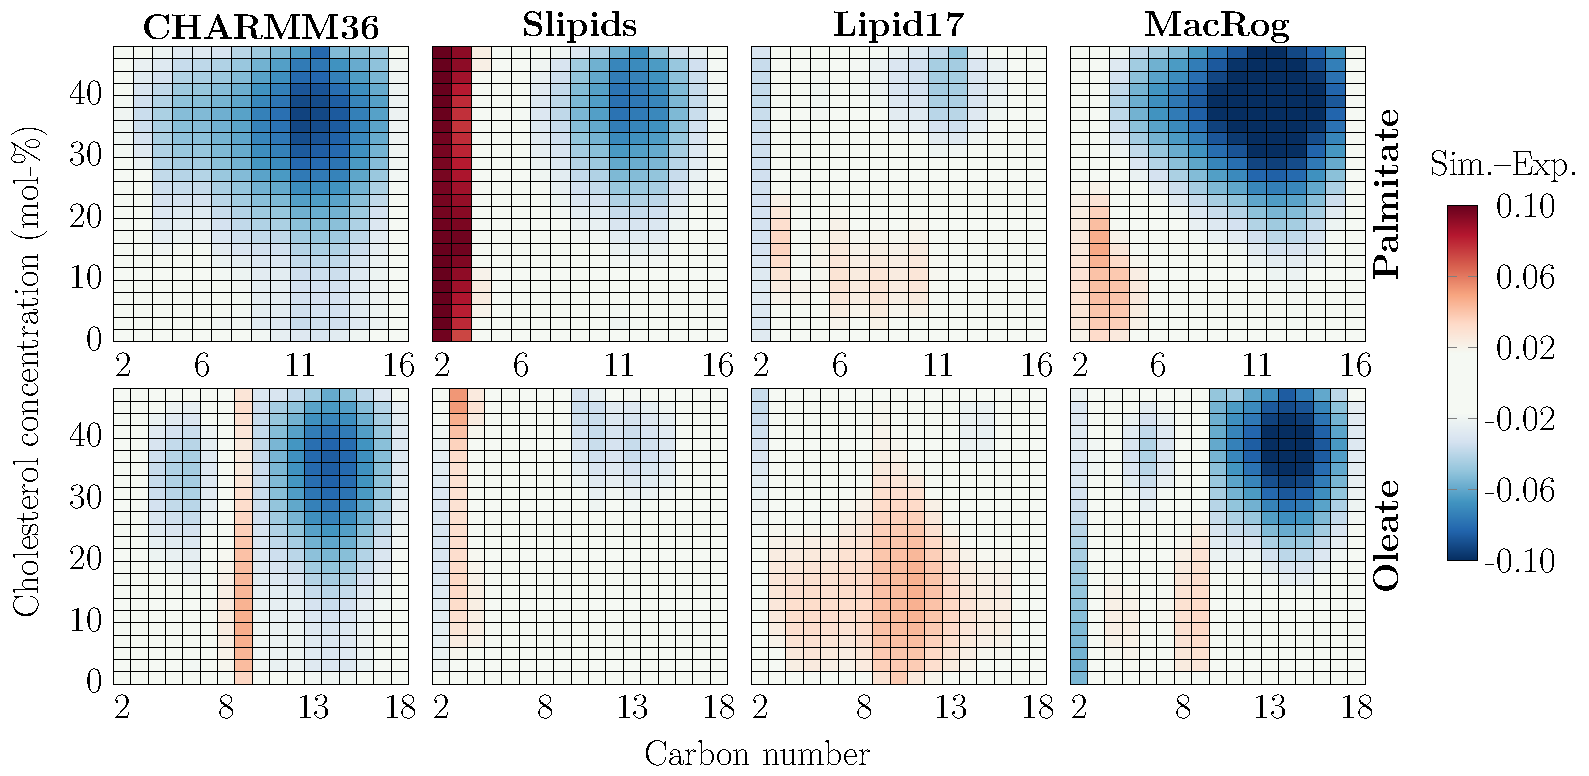
\includegraphics[width=\linewidth]{../FIGS/OP_chains.pdf}
  \caption{\label{fig:OPmaps}%
  POPC acyl chain order parameter deviation from experiments. Data are shown for palmitate (top row) and oleate (bottom row) and for the four force fields (columns). Negative values indicate that order is too high ($-S_\mathrm{CH}$ values too negative) in the simulations. The values that are within the estimated experimental error range of 0.02~\cite{ollila16} are coloured in white. Order parameters of identical hydrogens attached to the same carbons were averaged with the exception of C2 carbon of the oleate chain with the forked order parameters for which differences for both the larger and smaller values were calculated, and the average of this deviation is shown in the C2 column.
  }
\end{figure}

In CHARMM36, both the palmitate and oleate chains get too ordered upon increasing CHOL concentration. The oleate chain shows best agreement with experiment in Slipids, whereas there is some excess ordering in the palmitate chain. Still, the major discrepancy between Slipids and experiment is the drastically too disordered C2 and C3 carbons of the palmitate chain. This effect was introduced in the recent reparametrization of Slipids that improved the head group and glycerol backbone structures of Slipids \cite{grote2020optimization}. Lipid17 provides the best overall agreement with experiment, as no segments deviate significantly from experiment at any CHOL concentrations. MacRog behaves reasonably well at low CHOL concentrations, yet at larger CHOL concentrations the chains become overall way too ordered, leading to the largest overall deviations from experiment. For the head group and glycerol backbone order parameters, provided in Fig.~\ref{SIfig:headgroups}, CHARMM36 give the best agreement at all cholesterol concentrations in line with previous studies~\cite{botan15,antila2019headgroup}.

\subsection{Cholesterol Effect on Membrane Properties is Manifested Differently in Different Force Fields}

CHOL-induced ordering straightens the acyl chain conformations that leads to the thickening of membranes. While acyl chain order and membrane thickness are well correlated~\cite{NMRlipidsDatabank}, lipid bilayer dimensions can be accessed more directly by measuring X-ray scattering form factor, which is related to the electron density along membrane normal \textit{via} a Fourier transform \cite{pan12,Heftberger15,Marquardt15,ollila16}. Electron density profile, area per lipid and bilayer thickness can all be extracted from the form factor using the scattering density profile (SDP) model or its combination with MD simulations  \cite{Kucerka08a,pan12,Heftberger15,Marquardt15,doktorova2020molecular}. To complement the evaluation of CHOL ordering effect against NMR order parameters, we measured also X-ray scattering form factors from POPC--CHOL mixtures with systematically increasing CHOL concentrations. Scattering intensities from experiments are shown in Figs.~\ref{SIfig:scattering1} and \ref{SIfig:scattering2}, form factors from experiments and simulations in Fig.~\ref{SIfig:scattering}, and density profiles in Fig.~\ref{SIfig:densprofs}.


The effect of CHOL on structural properties of bilayers is compared between the SDP model (based on experimental form factors) and MD simulation results in Fig.~\ref{fig:densmaps}.  All force fields demonstrate increasing thickness upon addition of CHOL that saturates after approximately 30~mol-\% (bottom middle panel in Fig.~\ref{fig:densmaps}). MD simulations agree well with the SDP model below 30~mol-\% but overshoot the SDP results at high CHOL concentrations. Lipid17 simulations are exception as they predict thinner membranes than SDP model at low CHOL concentrations, and clear saturation of thickness increase is not observed, unlike for other force fields and experiments.

The dependence of APL on CHOL concentration follows the trends in thickness inversely in general (bottom right panel of Fig.~\ref{fig:densmaps}), yet provide curious differences between the force fields at the physiologically relevant CHOL concentration range \cite{van2008membrane}. Lipid17 has the largest APL across the entire CHOL contration range. MacRog also has a large APL for pure POPC, but the partial area of CHOL is negative until 30~mol-\% concentration indicating a particularly strong condensation effect. The profiles for Slipids and CHARMM36 are very similar with the small or zero CHOL partial area until a concentration of 20~mol-\%. 

\begin{figure}[htb!]
  \centering
  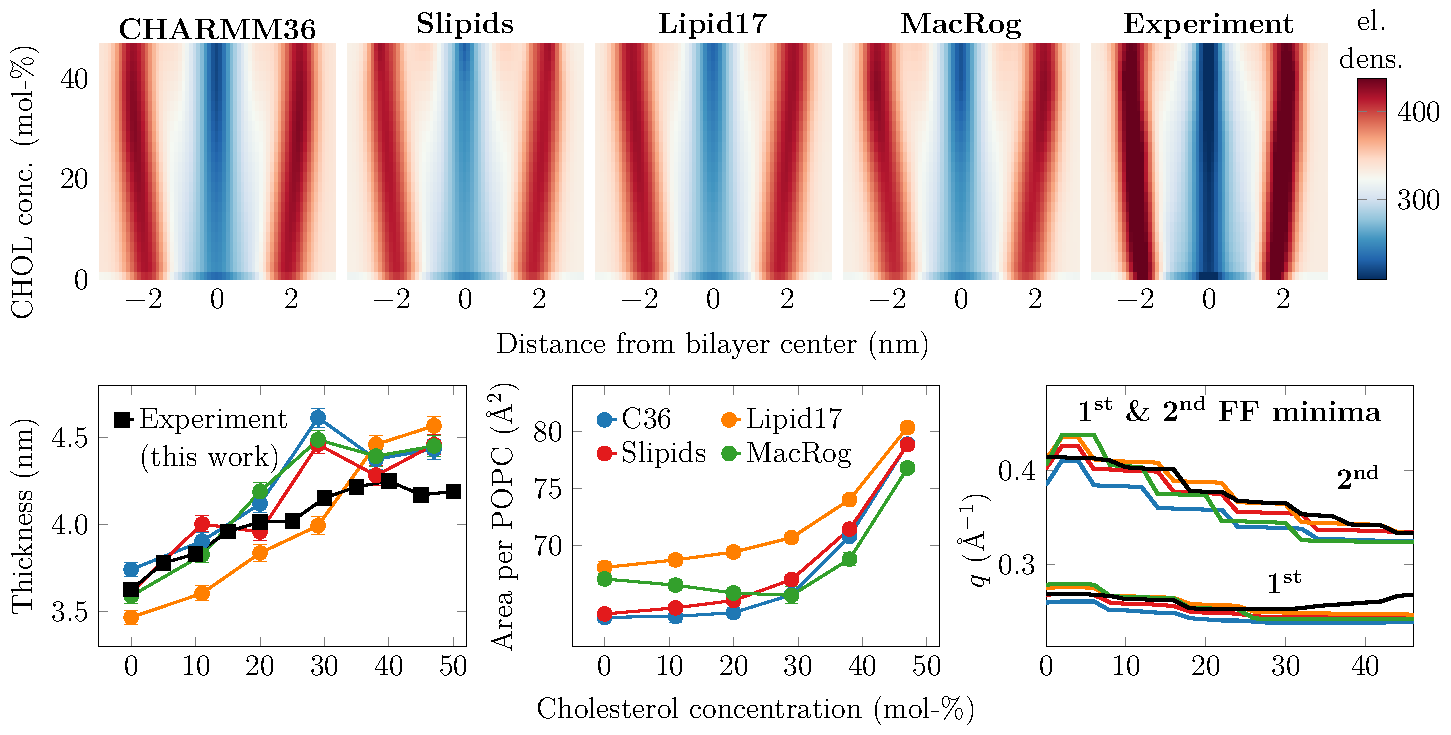
\includegraphics[width=\linewidth]{../FIGS/densitymaps.pdf}
  \caption{\label{fig:densmaps}%
  \textbf{Electron density profiles, thickness and area per lipid as a function of CHOL concentration.}
  %
  Top: Electron density maps for the simulations using four different force fields.
  %
  Bottom left: Electron density map for the experiment from the SDP model. The scaling is uniform between all simulations and experiment. The original electron density profiles are shown in Fig.~\ref{SIfig:densprofs}. The effect of system size on the density profiles in simulations is demonstrated in Fig.~\ref{SIfig:densprofssize} in the SI.
  %
  Bottom center: Bilayer thickness. Thickness is defined as twice the distance from the peak in electron density to the membrane core. Experimental data are extracted in a similar manner from electron density profiles obtained with X-ray scattering.
  %
  Bottom right: area per lipid measured by dividing the total membrane area by the number of phospholipids. The size-dependency of area per lipid is shown in Fig.~\ref{SIfig:aplvssize}.
  }
\end{figure}

For more detailed comparison of membrane structure, we interpolated the changes in electron density profiles along membrane normal (Fig.~\ref{SIfig:densprofs}) as a function of CHOL concentration to create two-dimensional electron density maps shown in Fig.~\ref{fig:densmaps}. Overall, all electron density profiles share the same features across all CHOL concentrations; a high-density band corresponding to the tightly-packed interfacial region containing electron-rich phosphorus, a low-density region at the core of the membrane occupied by the disordered acyl chains, and intermediate density in the rest of the lipid regions as well as the aqueous phase. However, a more detailed look at the profiles in Fig.~\ref{fig:densmaps} reveals differences between the force fields and SPD model. CHARMM36 has the sharpest low- and high-density bands among MD simulation results indicating smaller membrane fluctuations that would smear the bands, and the same is true for MacRog at higher CHOL concentrations. The less sharp bands for Lipid17 and especially Slipids profiles indicate that the membranes are more flexible with these force fields. SDP model gives the most sharp bands (bottom left panel in Fig.~\ref{fig:densmaps} and original electron density profiles in Fig.~\ref{SIfig:densprofs}), suggesting more uniform membrane structure than any MD simulation. However, System size plays a role here as  undulations smear out the density profile features with increasing simulation box size as demonstrated in Fig.~\ref{SIfig:densprofssize} by the density maps calculated for the CHARMM36 simulations in three sizes.  Still, even in the smallest system, the band intensities are less localized than in the SDP model. This difference might arise because most undulations are assigned to structure factor rather than form factor in their deconvolution, but it could also indicate different elastic properties between simulation and experiment.

Nevertheless, minima in X-ray scattering form factors are independent on simulation box size and correlate with membrane dimensions~\cite{NMRlipidsDatabank}. For more direct comparison between simulations and experiments, we thus interpolated the locations of first two minima in the form factors to the entire studied range of CHOL concentrations in the bottom right panel of Fig.~\ref{fig:deviation}. These curves highlight that the addition of CHOL first shifts the first minima to smaller wave vector values in the experiment, which is reasonably well captured by the simulation force fields. CHARMM36 seems to be off more than the other three force fields. Above $\sim$25~mol-\% of CHOL, the location of the minimum shifts to larger wave vector values in the experiment, which is curiously not captured by any of the force fields. The experiment shows a steady shift of the second minimum to smaller wave vector values, and this is reproduced by all simulation force fields. Slipids and Lipid17 are generally in better agreement with the experiment than MacRog and CHARMM36.


\subsection{The Force Fields Predict Very Different Lateral Mobilities}

Apart from the ordering effect on the bilayer structure, CHOL is also known to make them stiffer and less dynamic \cite{rog2009ordering,filippov2003effect,filippov2003influence}. The comparison between lateral diffusion coefficients extracted from simulation and experiment has been limited due to a box-size dependence observed in simulations performed using periodic boundary conditions \cite{vogele2016divergent,vogele2018hydrodynamics,camley2015strong}. Here, we tackle this issue by performing simulations with three system sizes, which allows the extrapolation of the results to an infinite system with the theoretical description developed by \citeauthor{vogele2016divergent} \cite{vogele2016divergent,vogele2018hydrodynamics}. The size-dependence of lipid lateral diffusion from simulations together with the fit of Eq.~\eqref{eq:sdlatpbc} are shown in Fig.~\ref{SIfig:dvssize}, whereas the CHOL-dependence of these values in systems with different sizes are shown in Fig.~\ref{SIfig:dvschol}. The PBC-corrected lateral diffusion coefficients are shown in the top panel of Fig.~\ref{fig:dynamics} together with experimental values from $^1$H pulsed field gradient NMR diffusion measurements on label-free macroscopically aligned bilayers~\cite{filippov2003influence,filippov2003effect}. 

\begin{figure}[htb!]
  \centering
  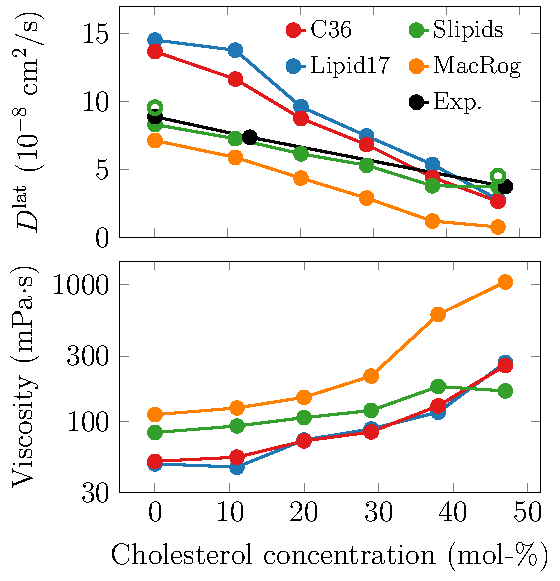
\includegraphics[width=8.7cm]{../FIGS/dynamics.pdf}
  \caption{\label{fig:dynamics}%
  \textbf{Dynamic properties of the POPC/CHOL mixtures.}
  Top: Lateral diffusion coefficients corrected for finite-size effects using Eq.~\eqref{eq:sdlatpbc}. Experimental data are taken from NMR measurements on well-hydrated samples \cite{filippov2003influence,filippov2003effect}. The hollow circles show data extracted for Slipids using a shorter Lennard-Jones cutoff (see text).
  %
  Bottom: Shear viscosities obtained from the finite-size correction, Eq.~\eqref{eq:sdlatpbc}.
  %
  The size-dependence of lateral diffusion and the fits used to obtain the PBC-corrected diffusion coefficients and shear viscosities are shown in Figs.~\ref{SIfig:dvssize} and \ref{SIfig:dvschol}.
  }
\end{figure}

The lipid force fields again show significantly different behavior. Lipid17 and CHARMM36 show too fast dynamics for pure POPC, and the slow-down induced by CHOL is exaggerated as compared to experiment. Diffusion in MacRog is generally too slow, yet Slipids provides an essentially quantitative agreement with experiment across the studied CHOL concentrations, and thus significantly outperforms other force fields in terms of lateral dynamics. Interestingly, there is no correlation between dynamic and structural properties described earlier when it comes to the deviations from experiments. To investigate if the differences in lateral diffusion coefficients could be explained by different Lennard-Jones (LJ) cutoff values, we repeated simulations at 0~mol-\% and 47~mol-\% CHOL for Slipids using a shorter cutoff of 0.9~nm corresponding to that of Lipid17, while original cutoff for Slipids was 1.4~nm (see Table~\ref{SItab:params}). The PBC-corrected diffusion coefficient values with shorter cutoff, shown in the top panel of Fig.~\ref{fig:dynamics} as hollow red circles, are only slightly larger than the original values, indicating that the LJ cutoff alone does not explain the differences between force fields, but they truly spark from differences in the force field interaction parameters.

When comparing lipid lateral diffusion between simulations and experiments, it is important to note that the PBC correction does not only affect values of diffusion coefficients but also qualitatively changes their trends as a function of cholesterol. This results from the fact that the size of the PBC correction, Eq.~\eqref{eq:sdlatpbc}, depends on membrane viscosity, which further depends on CHOL concentration. For example, Fig.~\ref{SIfig:dvschol} shows that Lipid17 and CHARMM36 systemically underestimate the experimental values in systems with all sizes simulated here while the effect of CHOL seems to be qualitatively reproduced. However, the PBC corrected values significantly overshoot the experiment at low CHOL concentration, and CHOL induces a more drastic slowdown in simulations leading to values close to experimental ones at 47~mol-\% CHOL. With MacRog, also the PBC corrected values fall below the experimental ones, yet the slowdown effect of CHOL again seems stronger than in experiment. With Slipids, the CHOL-dependence seems too weak with finite system sizes, yet after accounting for PBC effects, the agreement with experiment is excellent. These results highlight that little can be said about CHOL-dependence of lateral diffusion coefficients without performing simulations with multiple box sizes required for the PBC correction at different CHOL concentrations. Therefore, fine-tuning of interaction parameters to correctly reproduce lateral diffusion coefficients can require massive number of simulations.

We also provide the shear viscosity values of the membranes obtained from the fits of Eq.~\eqref{eq:sdlatpbc} in Fig.~\ref{fig:dynamics} for reference, yet they are not discussed further due to the large scatter of experimental estimates \cite{faizi2022vesicle}. Note that the data for CHARMM36 was also discussed in our previous work \cite{fabian2023protein}.

\subsection{Quality of Force Fields at Various Cholesterol Concentrations}

To streamline the selection of force fields that best capture the effect of CHOL on different membrane properties, we defined the quantitative quality measures for simulations. For this we calculated  relative deviations from experiments (difference of simulated and experimental values divided by the experimental value) using interpolated data for the form factor minima, the order parameters of the two acyl chains, and the diffusion coefficients from all the force fields. The quality evaluations are shown in Fig.~\ref{fig:deviation} for force fields that predicted different effects of CHOL on membrane properties in previous sections.

\begin{figure}[htb!]
  \centering
  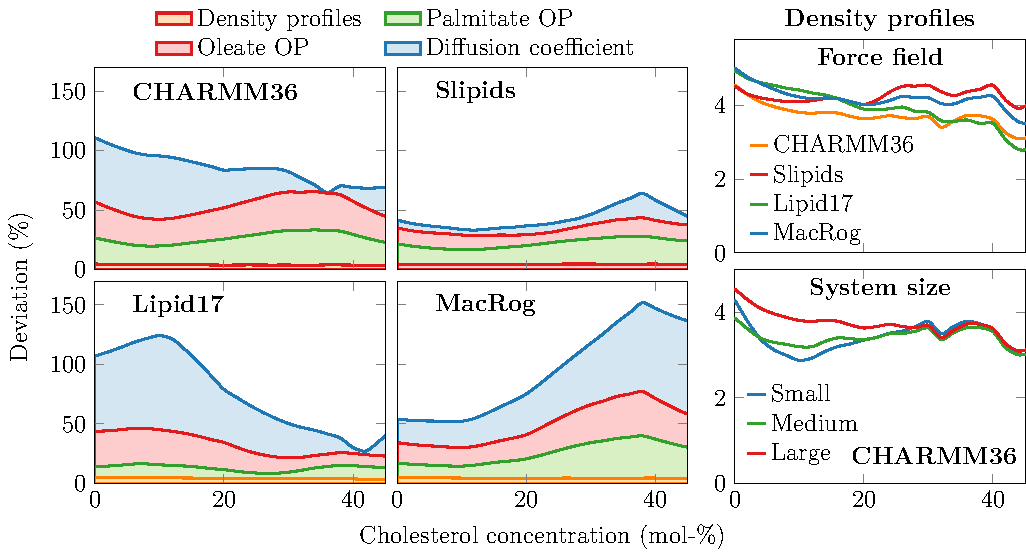
\includegraphics[width=\linewidth]{../FIGS/deviation.pdf}
  \caption{\label{fig:deviation}%
  \textbf{Total relative deviation of the force fields from experimental data.} 
%
  Two leftmost columns:
  The relative deviations from the first two minima in the form factor, palmitate and oleate chain order parameters, and diffusion coefficients are shown in a cumulative manner to highlight the overall deviation of the force fields from experimental data.
  %
  The order parameter deviations are obtained by averaging over the columns in Fig.~\ref{fig:OPmaps} and normalizing against experimental data. The differences in the form factor minima---shown in the bottom right panel---between experiment and simulation were calculated, normalized against experimental data, and summed together. The diffusion coefficient deviation is the difference of values from simulation and experiment in Fig.~\ref{fig:dynamics}, taken after interpolation to the same CHOL values as shown in Figs.~\ref{fig:OPmaps} and \ref{fig:densmaps}, and normalized against experimental values.
%
  Top right panel: 
  The zoomed-in view to the deviation in the location of the first minimum in the form factor.
%
  Bottom right panel:
  Effecf of CHOL on the location of the first two minima in the form factor. The minima are extracted from the form factors interpolated to all CHOL concentrations (Fig.~\ref{SIfig:scattering}) from experiment and simulation with the \texttt{findpeaks} function in Matlab.
  }
\end{figure}

The quality evaluations reveal that Slipids provides overall the best agreement with experiment, yet its quality decreases slightly at higher CHOL concentrations. Lipid17 provides a slightly better agreement with experiment above $\sim$30~mol-\% of CHOL than Slipids, but exhibits major deviation from experiments at low CHOL concentrations. MacRog performs relatively well at low CHOL concentrations, but its quality deteriorates significantly upon the addition of CHOL. The deviation metric for CHARMM36 are significant at all CHOL concentrations. 

Since the contributions from the form factor minima deviations are barely visible for some force fields in the leftmost columns of Fig.~\ref{fig:deviation}, we have highlighted the error in the 1\textsuperscript{st} minimum location in the top right panel of Fig.~\ref{fig:deviation}. This panel demonstrates that apart from CHARMM36, all force fields capture the location of the 1\textsuperscript{st} minimum relatively well at low CHOL concentrations, but deviate significantly at larger CHOL concentrations. 

\section{Conclusions}

The tested all-atom force fields captured the most important general effects of CHOL on membrane properties: increased acyl chain ordering, concomitant increase in bilayer thickness, and reduced lateral diffusion rate of lipids. However, quantitative comparison reveals differences between force fields and their qualities evaluated against NMR and X-ray scattering data. Comparison with NMR order parameters and X-ray scattering form factors propose that simulations reproduce experimental results up to 20~mol-\% of CHOL, but overestimate acyl chain ordering and membrane thickness after further addition of CHOL. An apparent exception to this is the Lipid17 force field, yet their seemingly better agreement with experiments can be explained by the over-correction of the originally underestimated acyl chain order at low CHOL concentrations upon CHOL addition. In conclusion, a unified picture emerging from comparison with NMR and X-ray scattering data suggests that all the tested force fields overestimate the CHOL ordering effect, particularly above 20~mol-\% of CHOL. Previously published comparison~\cite{ferreira13} suggests the same conclusion for historically relevant Berger/H{\"o}ltje force field parameters \cite{Berger97,Holtje01} that were not included in this work.

Besides the ordering effect, effect of CHOL on membrane properties has been discussed also in terms of the CHOL condensing effect which refers to a decrease in the \emph{area per phospholipid} upon the addition of CHOL (negative partial area) \cite{edholm2005areas}, or to CHOL having a diminishing partial area, meaning that a certain amount of CHOL could be added to a phospholipid bilayer without effecting its total area (zero partial area) \cite{javanainen2017two}. At the physiological CHOL concentrations in the range from 0 to 30~mol-\%, only MacRog predicts negative partial area for CHOL, while CHARMM36 predicts zero partial area, and Slipids and Lipid17 predict small positive partial areas. Considering that Slipids and Lipid17 perform best in our quality evaluation against experiments, yet still slightly overestimating the CHOL condensing effect, our results suggests that CHOL has a positive but small partial area.

Considering also lateral dynamics, Slipids is overall closest to experiments among the parameters tested here, and is therefore probably the best choice for studies where lipid--CHOL interactions play major role. Nevertheless, all tested parameters capture qualitative effects of CHOL on membrane properties relatively well and differences between force fields are clearly smaller than, for example, in the case of PC--PS lipid mixtures~\cite{antila2022emerging}. Therefore, the quality of selected force field for other molecules, such as, other lipids, proteins, sugars, or drugs, together with force field compatibility might be more relevant decisive factor for simulations of complex systems. Finally, it must be noted that while all simulations were performed with their suggested simulation parameters, the different simulation engines might provide slightly different behavior, yet we believe that evaluating the magnitude of these effects is well beyond the scope of this work.

Our results demonstrate that quality evaluation of lipid mixture simulations against experimental NMR and X-ray scattering data give consistent results for how accurately force field parameters capture intermolecular interactions. The interpolation approach introduced here extends the NMRlipids databank quality metrics~\cite{NMRlipidsDatabank} beyond individual systems enabling automatic ranking of not only lipid mixtures but also membrane mixed with other molecules such as ions. Such tools will strongly support the emerging endeavours for automatic improvements of force field parameters~\cite{antila2022emerging}.

\begin{suppinfo}
Simulation parameters used for all the studied force fields.
%
Form factor plots from simulations and experiments with the traced minima at various cholesterol concentrations.
%
Electron density profiles from simulation and experiment at various cholesterol concentrations.
%
Deuterium order parameters of both acyl chains of POPC from simulation and experiment at various cholesterol concentrations.
%
Deviation of POPC head group order parameters from experiment as a function of cholesterol concentration.
%
Lateral diffusion coefficients with varying cholesterol concentrations as a function of simulation box size from simulations together with the extrapolation of these values to an infinite box size.
%
Diffusion coefficients as a function of cholesterol concentration from simulations with varying box sizes together with comparison to experiment.
%
Effect of simulation box size on the area per lipid across the studied cholesterol concentrations.
%
Effect of simulation box size on the density profiles across the studied cholesterol concentrations.
%
Cholesterol tilt as a function of cholesterol concentration from simulations.
\end{suppinfo}

\begin{acknowledgement}
We acknowledge CSC -- IT Center for Science for computational resources.
%
%JJM thanks the Amber community (Benjamin Madej from the Walker lab and Callum Dickson from the Gould lab) for technical assistance related to the lipid14 force field parameters. 
%
MJ (grant no. 338160) and OHSO (grant nos. 315596 \& 319902) thank the Academy of Finland for funding.

\end{acknowledgement}

\bibliography{refs.bib}

\end{document}
